\documentclass[12pt]{article}
\usepackage[a4paper,top=24mm,bottom=24mm,left=24mm,right=24mm]{geometry}
\usepackage{fontspec}
\setmainfont{[Times-New-Roman-400.ttf]}
\linespread{1.25}


\usepackage{array}
\usepackage{longtable}
\usepackage{graphicx}
\usepackage{blindtext}
\usepackage{dirtytalk}
\usepackage{xcolor}
\usepackage{listings}
\usepackage[english]{babel}
\usepackage{comment}

\renewcommand{\tt}{\texttt}
%\newcommand{\ctt}{#1}{\begin{center}\texttt{#1}\end{center}}

\title{Report \\ Group 2}

\date{January 2020}

\definecolor{dkgreen}{rgb}{0,0.45,0}
\definecolor{gray}{rgb}{0.5,0.5,0.5}
\definecolor{mauve}{rgb}{0.30,0,0.30}


% Default settings for code listings
% Default settings for code listings
\lstset{frame=tb,
  language=C,
  aboveskip=3mm,
  belowskip=3mm,
  showstringspaces=false,
  columns=flexible,
  basicstyle={\small\ttfamily},
  numbers=left,
  numberstyle=\footnotesize,
  keywordstyle=\color{dkgreen}\bfseries,
  commentstyle=\color{dkgreen},
  stringstyle=\color{mauve},
  frame=single,
  breaklines=true,
  breakatwhitespace=false
  tabsize=1
}

\begin{document}

\begin{titlepage}
    \begin{center}
        \vspace*{-2cm}\hspace*{1cm}
 
        \vspace{2.5cm}


        {\let\newpage\relax\maketitle}
        \thispagestyle{empty}

        \vspace{0.8cm}

        \begin{minipage}{.8\textwidth}
        Hello
        \end{minipage}

    \end{center}
\end{titlepage}


\newpage

% https://tex.stackexchange.com/a/291312
\setcounter{tocdepth}{2}
\tableofcontents
\newpage

% The structure below is a guideline for the project description. The main sections are given in the following list. Feel free to insert subsections as you see fit.

% 1 - Introduction. This section gives an overview of the motivations and results of what you have done. Describe the challenge that you want to address, motivating why it is relevant.

% 2 - Preliminaries. Give a brief overview of the background knowledge needed to understand your report. Provide references to what you have used and report the main concepts that your work is based on.

% 3 - Technical Description. Here you explain the technical work you have carried out. You may include code snippets where relevant, and refer to source code in the project files. Try to explain the development choices you did taking into account important properties such as deployability, availability, reusability, security, modifiability, performance.

% 4 - Related Work and Discussion. In this section you review the relevant state of the art. This may include alternative solutions to the same challenge you have tried to address in your project, or alternative methodologies that you may have followed (e.g., choice of other technologies for implementing the project). Provide a discussion on the implications of your choices in the design of your work and the technologies/techniques that you have used.

%     References (or Bibliography) This section should contain references to the articles/websites/resources/etc. cited in your report.


% 1 - Introduction. This section gives an overview of the motivations and results of what you have done. Describe the challenge that you want to address, motivating why it is relevant.

\section{Introduction}\label{sec:introduction}
The purpose of this project has been to develop a chat application that allows its users to automate in- and outbound messages,  through user uploaded scripts written in the service oriented programming language, Jolie, while maintaining security.

The underlying infrastructure of the application itself has been built as a micro-service architecture with the goal of affording developers greater atonomy and agility in the limited scope that they are responsible for.

The choice of a micro-service architecture also helps another key goal, namely that of good horizontal scalability; we have utilized the venerable container orchestration framework, Kubernetes to facilitate this. Every service is containerized using Docker, and managed as pods in Kubernetes.
% 2 - Preliminaries. Give a brief overview of the background knowledge needed to understand your report. Provide references to what you have used and report the main concepts that your work is based on.

\section{Preliminaries}\label{sec:preliminaries}
In this section we will provide an overview of the concepts, tools and platforms that we have used and what they are.
\subsection{Containerization}
Containerization is the concept of packaging the environment your application needs with the application itself into a small self-contained package.
In our project we have used Docker for this.
\subsection{REST}
REST is an API spec, that is built ontop of HTTP. We use REST for interacting with our service from the outside, since it is almost an ISO standard for how to expose your web-services.
\subsection{Kubernetes}
Kubernetes is a self-healing, fast, fault-tolerant, and pluggable spec, for container orchestration and networking abstraction at scale.
\subsubsection{Self-healing}
In the context of kubernetes, self-healing means that the kubernets master actively makes sure that containers are healthy, if not they are restarted (usually).
\subsubsection{Fast}
Kubernetes services are usually configured at one of the networking layers, making it extremely fast, and runtime-configurations is implemented at systemcall-level.
The whole system is also written in Go, which is known to have very good performance.
\subsubsection{Pluggable}
Kubernetes itself is more of an api that usually has pre built-in modules.
An example is the kube-dns, which can easily be plugged with another DNS.
The kubernets ingress controllers can also be plugged for something like nginx, if chosen to.
\subsubsection{Container orchestration}
Usually people know this by automatic scheduling and resource management for containers.
Imagine having 3 virtual machines and 50 containers, kubernetes automatically handles all the deploying and networking for you.
\subsection{Prometheus}
Prometheus is a applications monitoring spec, like JVM memory details, Go garbage collector details and much much more.
It is also a server software, that can pull from REST endpoints (usually /prometheus), and then exposes another api with all the collected data that can be consumed by eg Grafana.
\subsection{Grafana}
Grafana is a visualization tool, it can be connected to various sources (such as prometheus and loki), for data visualization.
\subsection{Loki}
Loki is a brand new software from the grafana team, that harvests logs stores them in cassandra and tokenizes them for extremely fast lookup.
Loki exposes an endpoint that adheres to the prometheus spec, so it is also extremely pluggable.
\subsection{Redis}
Redis is an extremely high-performance in-memory simple key-value store but extensible through an plugin environment.
Redis is used often for query caching and session management.
\subsection{Postgres}
Postgres is a state of the art high performance RDBMS.
\subsection{Kafka}
Kafka is a fully distributed, pub-sub like messaging system that employs log techniques instead of the ordinary ack-pop of pub-sub systems.
Kafka is the most widely used modern messaging system of it's category of pub-sub systems.
\subsection{JSON}
JSON is a data modelling language, it is simple and easy to read.
\subsection{JWT}
JWT stands for Json-Web-Token, which is a method of dispensing authentication tokens to users.
\subsection{GCS}
GCS stands for google cloud storage, its a thirdparty object storage service from google cloud.
% 3 - Technical Description. Here you explain the technical work you have carried out.
% You may include code snippets where relevant, and refer to source code in the project files.
% Try to explain the development choices you did taking into account important properties such as deployability, availability, reusability, security, modifiability, performance.

\section{Technical Description}\label{sec:technicalDescription}
In this section the technicalities of the project is explained.
First the spec will explained and then every aspect into more detail.
A flowchart of the stack can be seen below:\\
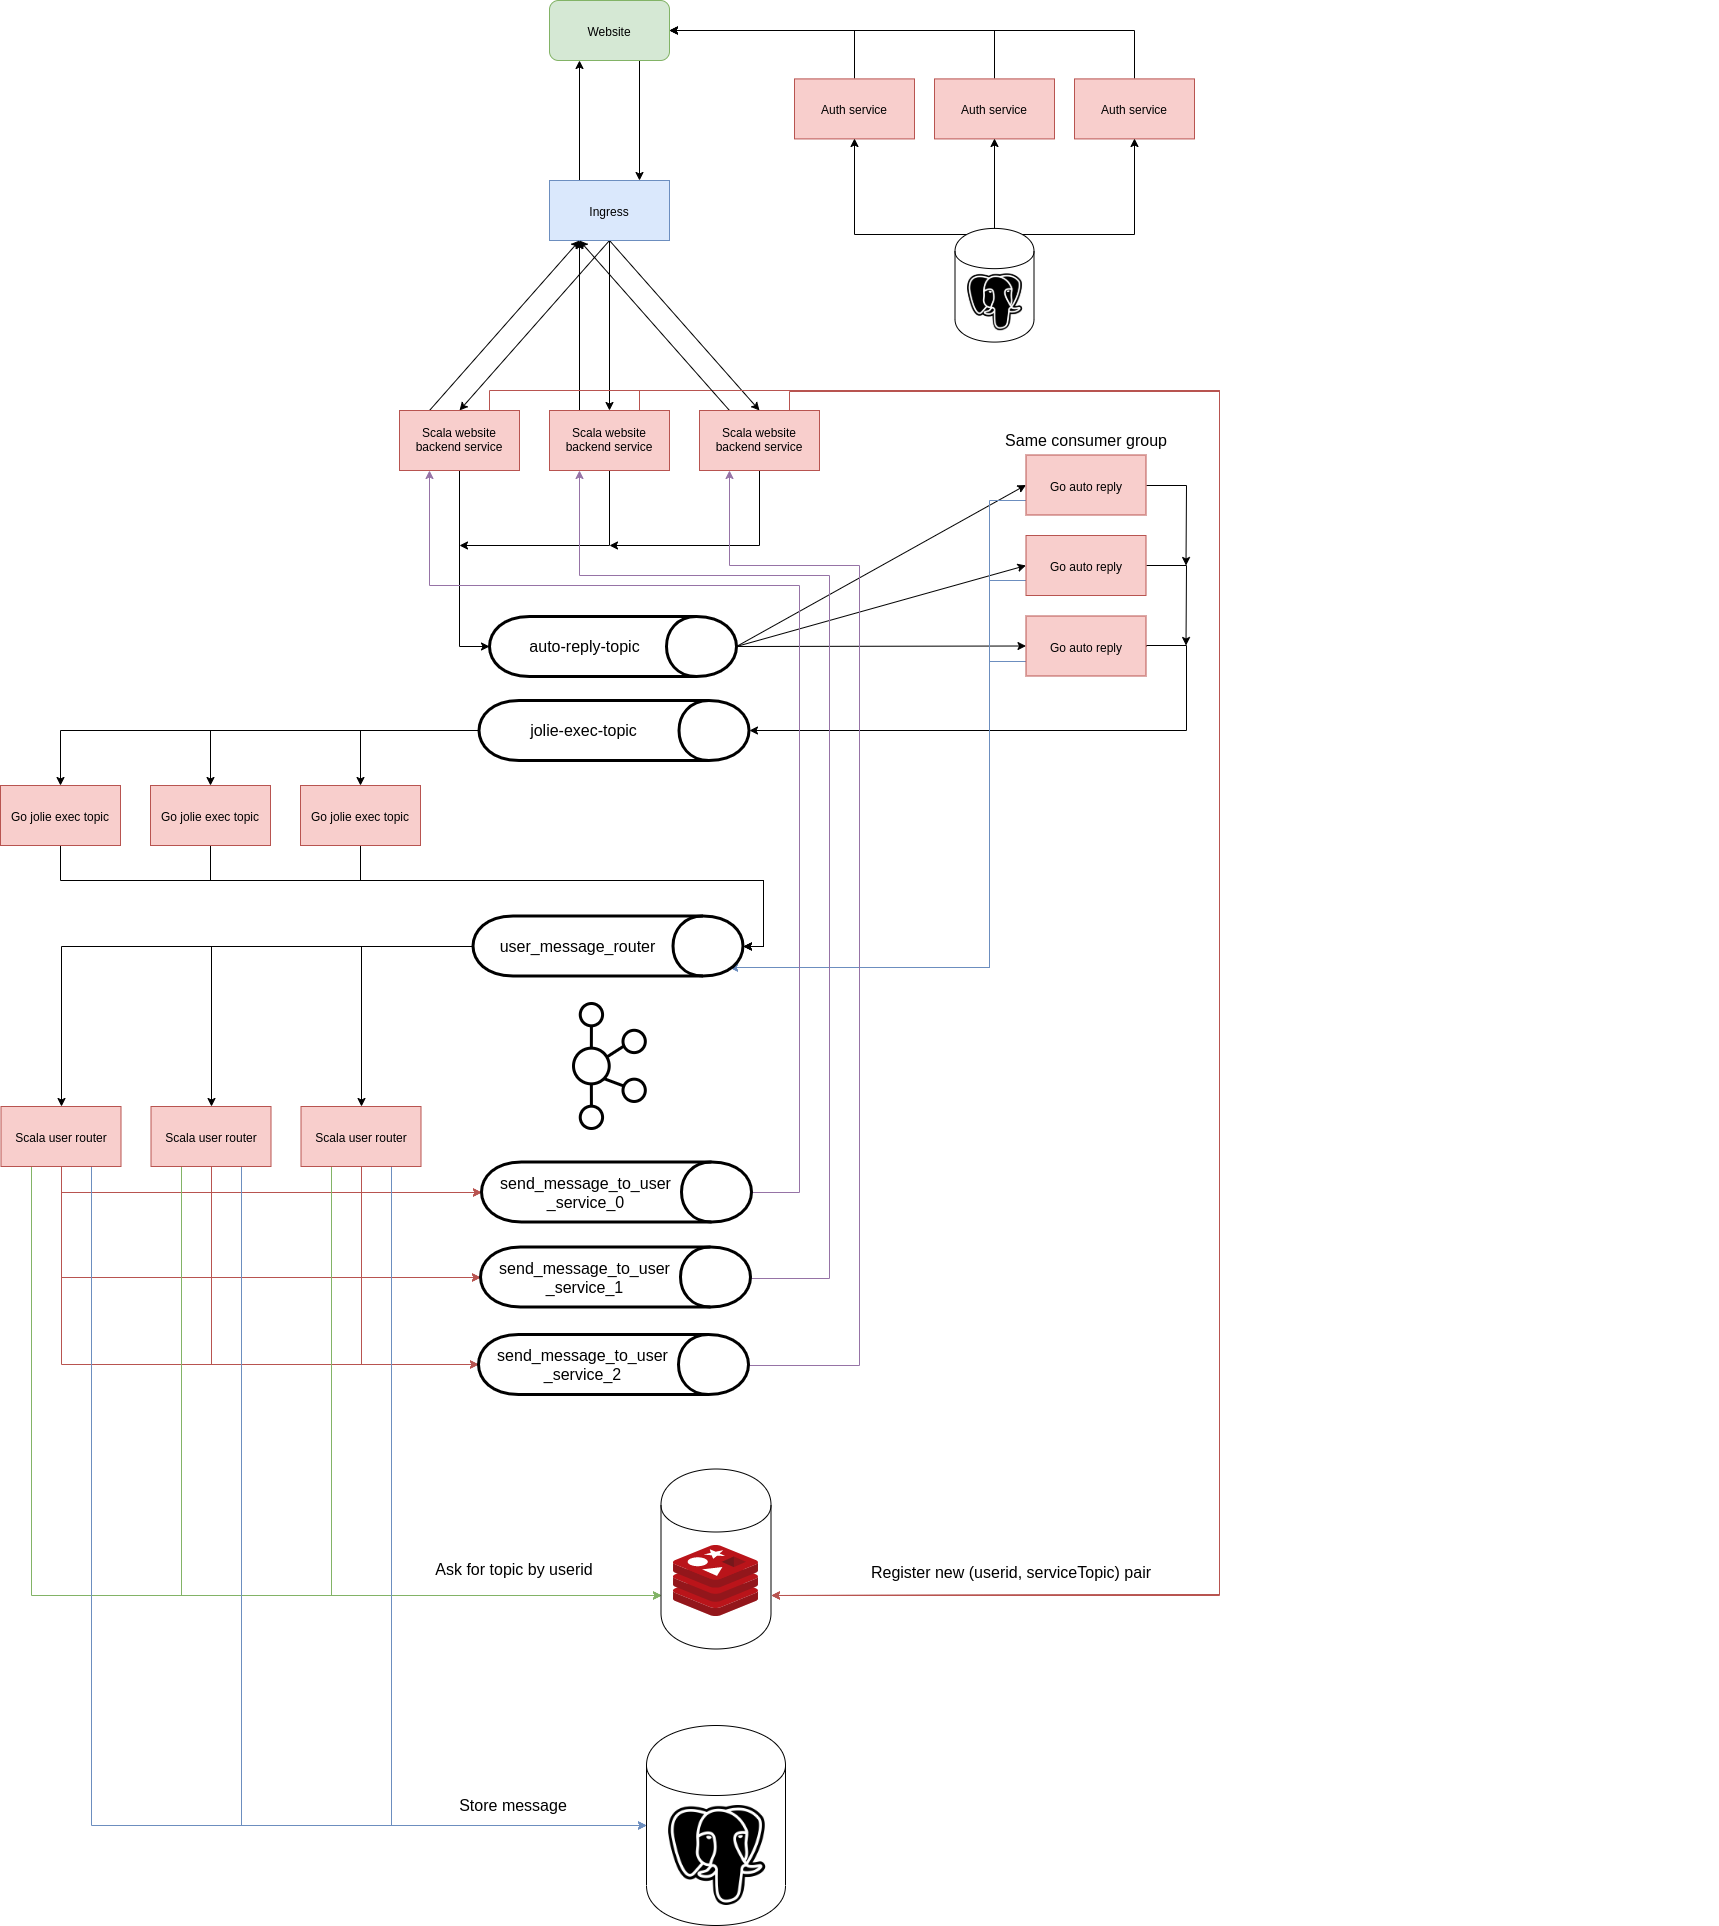
\includegraphics[scale=0.38]{stack.png}
\\
In the spec we use an event sourcing like technique.\cite{fowlerEventSourcing}
This includes a stateful data-structure that every service knows the structure of.
This structure contains any data about a message that a service would need to know, as well as the sender user.\\
\begin{lstlisting}
    {
        "messageUid": "c0a630d2-8db3-4a03-9e19-7141582f37aa",
        "sessionUid": "cf2bd7ca-ba13-40d9-8fb7-bab2064028d4",
        "messageBody": "Hello, world!",
        "senderId": 42,
        "recipientIds": [12, 8],
        "fromAutoReply": false,
        "eventDestinations": ["TOPIC1", "TOPIC2"]
    }
\end{lstlisting}
\begin{enumerate}
    \item \texttt{messageUid} a UUID that represents the message id.
    \item \texttt{sessionUid} a UUID to represent the user session (websocket session).
    \item \texttt{messageBody} this is the full message.
    \item \texttt{senderId} this is the user id of the sender.
    \item \texttt{recipientIds} these id's represent the recipient user id's.
    \item \texttt{fromAutoReply} this represents if the message was generated through pragmatic methods.
    \item \texttt{eventDestinations} this represents the topics (services) that the message must go through, usually a message ends in the router.
\end{enumerate}

\subsection{Microservices}
This section covers the responsibilities and design choices of the different microservices that comprise the chat application.

\subsubsection{Webserver (website backend)}
This service has 5 simple but important objectives.
\begin{enumerate}
    \item To serve the static single page React application.
    \item To handle user websockets through the kubernetes ingress \& insert itself as the manager of a user websocket.
    \item To check authentication when a user makes a request.
    \item To "bootstrap" a message, by inserting into one of these event sourcing models (see the JSON structure in above).
    \item To route messages back to the recipient user websockets.
\end{enumerate}
The service is written in scala and is independently scalable, has no state, storage or any stateful requirements.
It is fault tolerant and secure through JWT using HMAC256 symmetric private key encryption.

\subsubsection{Auto reply}
The auto reply service is an internal (to the cluster) service responsible for providing users with a simpler alternative to writing Jolie scripts to automate replying to messages. The feature works like how auto reply does in most e-mail clients; letting users write a static message that will be sent to everyone trying to message them. The message can be toggled on or off in the settings of the chat application.

The service is written in the Go programming language, which lends itself well to microservice development for a few reasons:

\begin{itemize}
	\item It is modern enough to have many built-in facilities useful for micro service development, like easy JSON encoding and decoding.
	\item It is a compiled language which means the service will require fewer hardware resources for the same performance.
	\item It is a strongly typed language which helps catch many bugs during compilation.
	\item Since it is developed by Google who themselves use a microservice architecture for many of their services, there exists many tools and resources for containerizing go applications and deploying them with Kubernetes which also happens to be by Google.
\end{itemize}

\subsubsection{Jolie exec}
\subsubsection{Router}
The router service is responsible for routing messages to the correct services, eg the one managing the websocket for the recipient user.
The router service simply makes a lookup in redis for the key of the self-registered managed websocket, and sends the message to the found web-servers.
% static services
\subsection{Deployability}
We have chosen to use kubernetes for this project to manage almost all of our deployability.
One of the key points of kubernetes is that if your deployment configurations are written well, it handles all deployment oriented aspects.
Kubernetes is an extension to containerization, and since containerization envisions the idea of easy deployments kubernetes really pushes it to the next level.

All runtime aspects and configuration has deployability and scalability in mind, using many built-in parts of kubernetes.
We have the flexibility to say here is a service and it's configuration (which is dynamically injected at runtime if changed), now run it.
\subsection{Reusability}
Reusability is employed on two different levels.
One is the level that we re-use Kafka for every aspect of cross-service communication, meaning that kafka is the only pre-requisite to understand the communication model.

On the other side, we have services with clear API definitions.
These services can be chained in any order chosen, thus they are completely reusable if the message flow needs it.
\subsection{Performance}
Performance was a big part of our considerations, both in designing the system and the physical performance.
One of the most important parts of performance is the ability to do scaling seamlessly.
An instance of this is how we introduced a router service and a redis instance to remove the need to check all websocket managers if they managed a connection to whatever user was receiving a message.

All services are completely stateless and scalable except the websocket manager (webserver) instance, since it needs to do some rebalancing if a downscale must happen.
All services are also written in high performance asynchronous languages, which include Go and Scala.

The idea of introducing kafka has also been for performance aspects, since kafka has an obscene throughput (at least 100k req/sec without message bulking).
\subsection{Fault tolerance}
Since we have chosen to use Kafka for this project, we basically get fault tolerance for free.
Kafka is fully distributed and might be one of the most fault tolerant pieces of software out there.
It uses >2 instances of apache zookeeper, a distributed store (basically a filesystem structure) to manage the Kafka metadata.
Kafka has the ability to have multiple brokers (brokers just means instances) crash and still go on as if nothing has happened.
It uses leader election and built-in heartbeat methods which also the producers and consumers know of when connecting, and has automatic load balancing through broker rebalancing.

As stated earlier all services are completely stateless (again, escept the websocket manager), so it compliments Kafka to keep track of the messages, since Kafka is more of a log store than a traditional pub-sub.
\subsection{Monitoring}
For monitoring the system we have chosen to go the opensource, modern and standardized way with Prometheus, Grafana and Loki.
These three are an equivalent of the ELK stack, but seem to have much less resource requirements and be less of a pain to maintain.
We have used public Grafana dashboards for Kafka and Kubernetes monitoring:\\
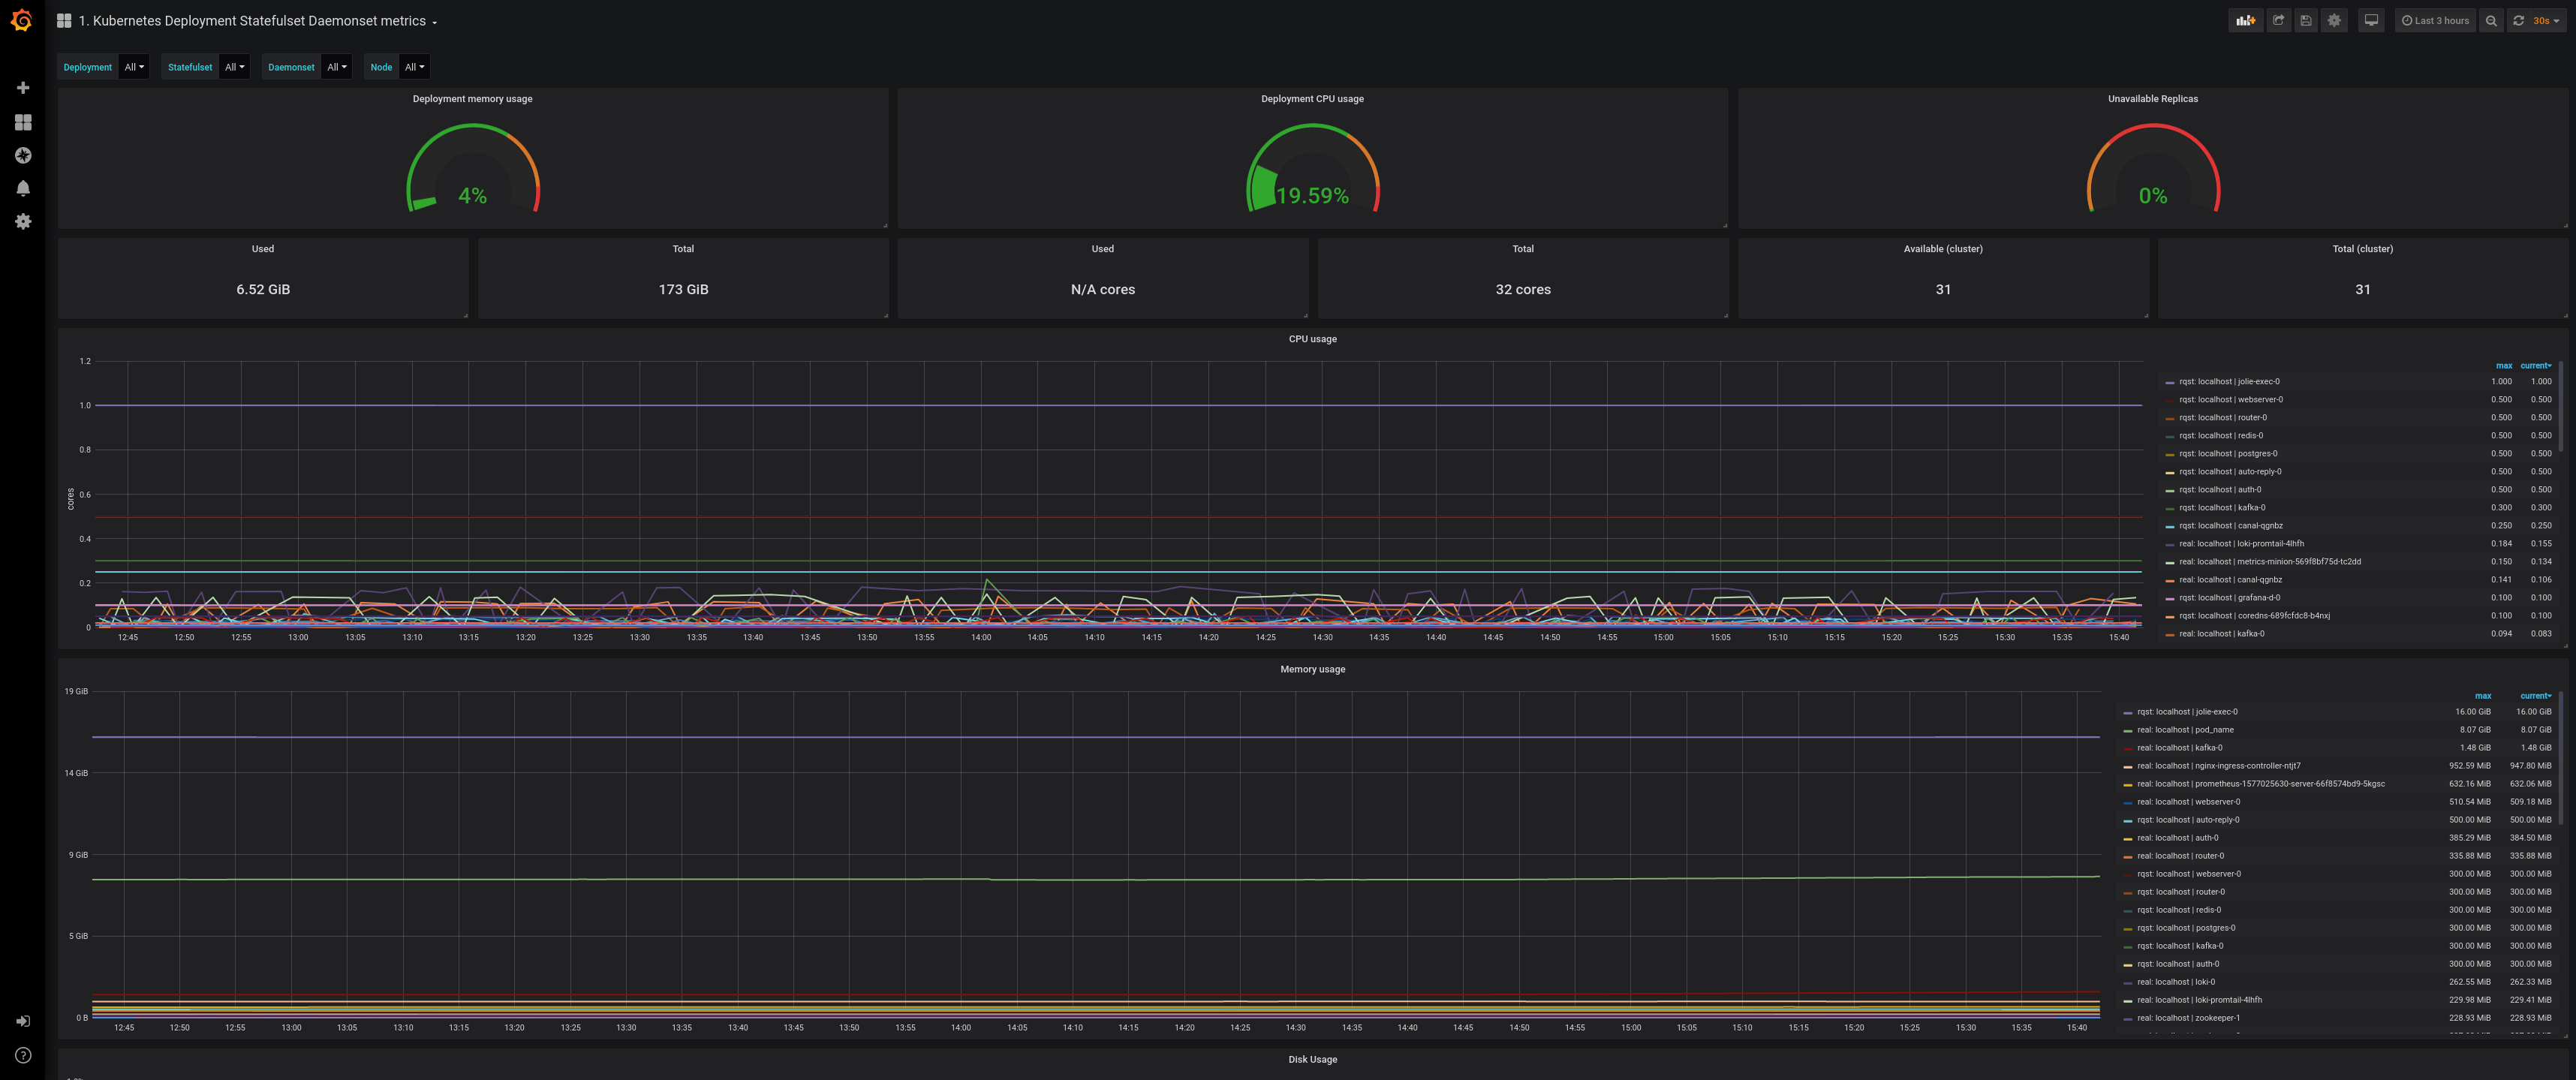
\includegraphics[scale=0.133]{grafana.png}\\
And Loki is purely log aggregation:\\
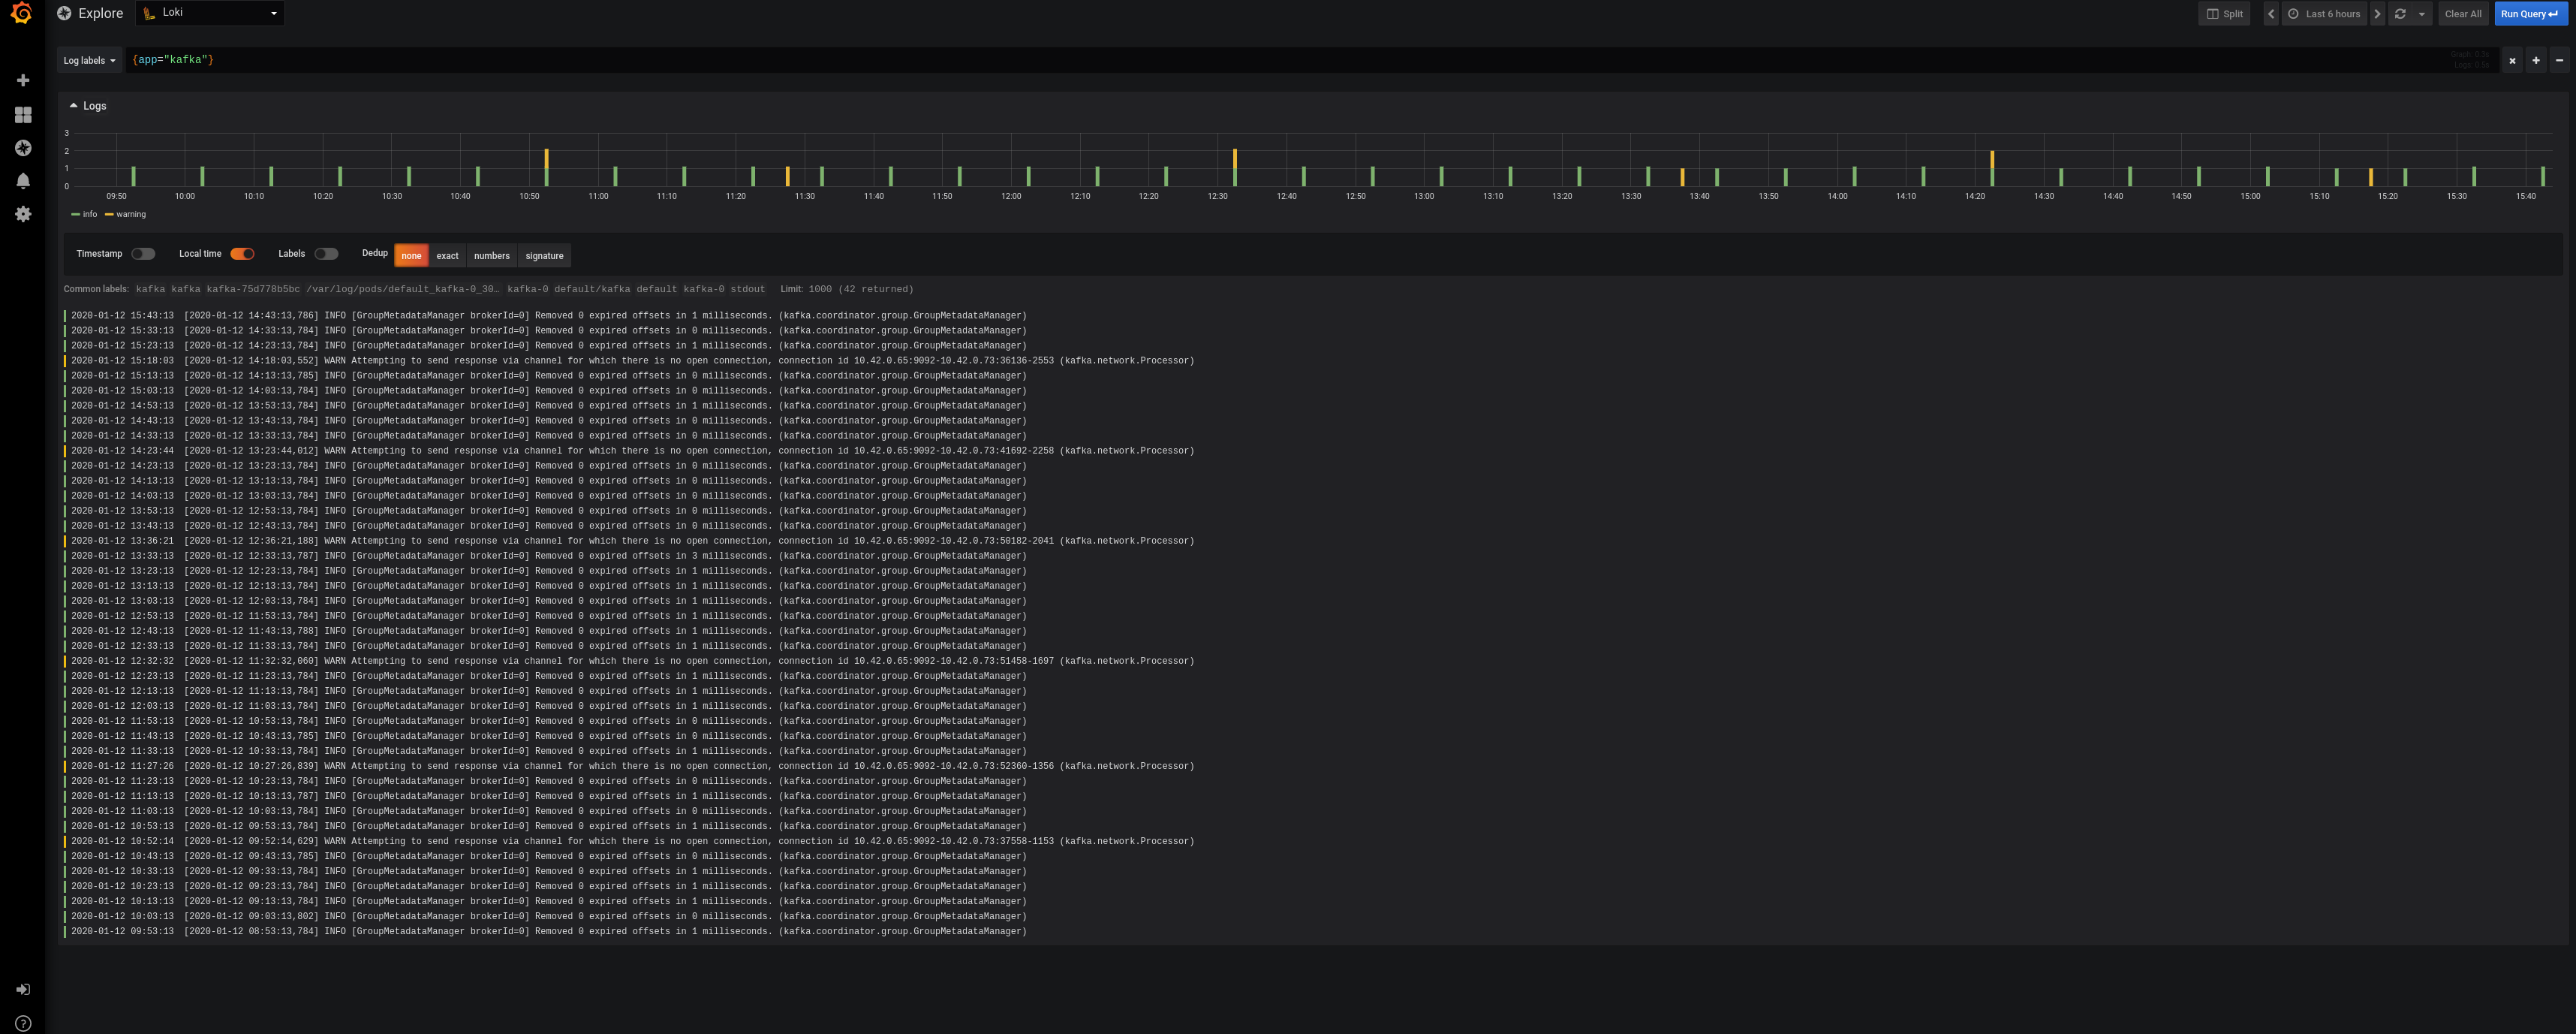
\includegraphics[scale=0.133]{loki.png}\\

% 4 - Related Work and Discussion. In this section you review the relevant state of the art. This may include alternative solutions to the same challenge you have tried to address in your project, or alternative methodologies that you may have followed (e.g., choice of other technologies for implementing the project). Provide a discussion on the implications of your choices in the design of your work and the technologies/techniques that you have used.

\section{Related Work and Discussion}\label{sec:relatedWorkAndDiscussion}

-- related work limited as the project was about using already well known technologies together
-- alternatives to jolie (resource cost wise)
-- kafka vs REST
%     References (or Bibliography) This section should contain references to the articles/websites/resources/etc. cited in your report.

\section{References}\label{sec:references}
\begin{otherlanguage}{australian}
\printbibliography[heading=none]
\end{otherlanguage}

\clearpage

\newpage


\end{document}
